\documentclass[12pt]{article}
\usepackage[margin=2.5cm]{geometry}
\usepackage{enumerate}
\usepackage{amsfonts}
\usepackage{amsmath}
\usepackage{fancyhdr}
\usepackage{amsmath}
\usepackage{amssymb}
\usepackage{amsthm}
\usepackage{mdframed}
\usepackage{graphicx}
\usepackage{subcaption}
\usepackage{adjustbox}
\usepackage{listings}
\usepackage{xcolor}
\usepackage{courier}
\usepackage[utf]{kotex}
\usepackage{hyperref}
\usepackage{soul}
\usepackage{cancel}


\definecolor{codegreen}{rgb}{0,0.6,0}
\definecolor{codegray}{rgb}{0.5,0.5,0.5}
\definecolor{codepurple}{rgb}{0.58,0,0.82}
\definecolor{backcolour}{rgb}{0.95,0.95,0.92}

\lstdefinestyle{mystyle}{
    backgroundcolor=\color{backcolour},
    commentstyle=\color{codegreen},
    keywordstyle=\color{magenta},
    numberstyle=\tiny\color{codegray},
    stringstyle=\color{codepurple},
    basicstyle=\ttfamily\footnotesize,
    breakatwhitespace=false,
    breaklines=true,
    captionpos=b,
    keepspaces=true,
    numbers=left,
    numbersep=5pt,
    showspaces=false,
    showstringspaces=false,
    showtabs=false,
    tabsize=1
}

\lstset{style=mystyle}

\pagestyle{fancy}
\renewcommand{\headrulewidth}{0.4pt}
\lhead{CSC 369}
\rhead{Tutorial Notes}

\begin{document}
\title{CSC 369 Tutorial Notes}

\begin{enumerate}[1.]
    \item \texttt{ls /tmp/mount/dir2} calls the following:

    \bigskip

    \texttt{getattr(/dir2, 0x7f2cebffec30)}\\
    \texttt{readdir(/dir2, 0x7f2cec0016b0)}\\
    \texttt{getattr(/dir2/newfile, 0x7f2cf0c48c30)}

    \item \texttt{passthrough\_utimens} is called using the following list of commands

    \begin{itemize}
        \item \texttt{touch /tmp/hyungmo/dir1} (when directory \texttt{dir1} already exists)
        \item \texttt{touch /tmp/hyungmo/newfile} (when file \texttt{newfile} doesn't exist)
        \item \texttt{touch /tmp/mount/afile} (when file \texttt{afile} already exists)
    \end{itemize}

    \item \texttt{cd /tmp/hyungmo/dir1} is called, the following functions are run

    \begin{itemize}
        \item \texttt{getattr}
    \end{itemize}

    \item FUSE doesn't detect passthrough code created in \texttt{rootdir/dir1}

    \bigskip

    \color{red}NOTE\color{black}: None detected when a file is created through \texttt{rootdir}

    \bigskip

    \item Creating a file in \texttt{/tmp/hyungmo/dir1} can be seen through \texttt{rootdir}

    \begin{center}
    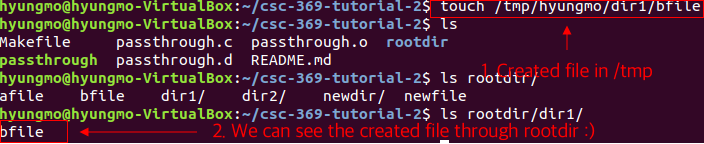
\includegraphics[width=0.8\linewidth]{images/notes_15.png}
    \end{center}

    \item \texttt{passthrough\_rename} is called using \texttt{mv} command
    \item On creating a non-empty file in \texttt{tmp/hyungmo}, two files are created

    \begin{itemize}
        \item \texttt{bfile}
        \item \texttt{/.bfile.swp}
    \end{itemize}


    \item Just running \texttt{nano /tmp/hyungmo/bfile} invokes the following system calls

    \begin{itemize}
        \item \texttt{create}
        \item \texttt{getattr}
        \item \texttt{write}
    \end{itemize}

    \item Writing words, saving and exiting in \texttt{nano /tmp/hyungmo/bfile} invokes the following system calls:

    \begin{itemize}
        \item \texttt{getattr}
        \item \texttt{create}
        \item \texttt{unlink}
        \item \texttt{write}
    \end{itemize}

    \item Accessing \texttt{nano /tmp/hyungmo/bfile} invokes the following system calls

    \begin{itemize}
        \item \texttt{getattr} (from \texttt{bfile} and \texttt{.bfile.swp})
        \item \texttt{create} (from \texttt{.bfile.swp})
        \item \texttt{read} (from \texttt{bfile})
        \item \texttt{write} (from \texttt{.bfile.swp})
    \end{itemize}

\end{enumerate}

\end{document}
